\documentclass[12pt]{mwart}
\usepackage{polski}
\usepackage[utf8]{inputenc}
\usepackage[T1]{fontenc}
\usepackage{lmodern}
\usepackage{mathtools,amsthm,amssymb,icomma,upgreek,xfrac,enumitem,multicol,paracol}
%\usepackage[hidelinks,breaklinks,pdfusetitle,pdfdisplaydoctitle]{hyperref}
\usepackage{cancel}
\mathtoolsset{showonlyrefs,mathic}
\title{\textbf{Raport 1.}}
\author{\fontsize{12pt}{12pt}\selectfont \emph{Klaudia Janicka, 262268, Julia Mazur, 262296}}
\date{30 kwietnia 2022r.}
\usepackage{float}
\usepackage{extsizes}
\usepackage[margin=0.3in]{geometry}

\setlist[enumerate]{}
\setlist[itemize]{itemsep=0.3em}

\DeclareMathOperator{\diff}{d\!}

\begin{document}
	\maketitle
	\section{Cele}
	\begin{itemize}
		\item[$\bullet$] Analiza dokładności otrzymanych wartości pojemności kondensatorów podczas mierzenia czasu ładowania i~rozładowania kondensatora.
		\item[$\bullet$] Analiza wpływu zmiany parametrów $\alpha$ i $\beta$ na~dokładność otrzymanych pojemności kondensatora.
	\end{itemize}
	\section{Wstęp teoretyczny}
	\noindent Aby wyprowadzić równanie różniczkowe i~następnie wyznaczyć czasy ładowania i~rozładowania, korzystamy~z:
	\begin{itemize}
		\item[$\bullet$] prawa Ohma
		\item[$\bullet$] I prawa Kirchhoffa
		\item[$\bullet$] II prawa Kirchhoffa
	\end{itemize}
	Dzięki nim otrzymujemy, że 
	
	\begin{equation}\label{row_roz}
		\frac{\diff U_{c}}{\diff t} +\frac{1}{RC}\, U_{c}=\frac{U}{RC},
	\end{equation}
	gdzie $U_{c}$ to~napięcie na~kondensatorze $\left[V\right]$, $R$, to~opór $\left[\Omega\right]$, $C$ to~pojemność kondensatora $\left[F\right]$, a~$t$ to~czas.
	Czas ładowania możemy wyznaczyć na~podstawie rozwiązania \ref{row_roz}, przyjmując początkowy stan naładowania kondensatora~jako $\alpha U$ a~końcowy~jako $\beta U$, zakładając, że~$0 < \alpha < \beta < 1$. Wtedy możemy wyznaczyć pojemność kondensatora~jako $$C=\frac{t_{c}}{R\,ln\left(\frac{1-\alpha}{1-\beta}\right)}.$$\label{poj_lad}
	\phantom{a}\\
	Aby rozładować kondensator nie dostarczamy mu już napięcia, zatem $U = 0$, a wtedy równanie \ref{row_roz} staje się równaniem jednorodnym
	\begin{equation}\label{row_roz2}
		\frac{\diff U_{c}}{\diff t} +\frac{1}{RC}\, U_{c}=0.
	\end{equation}
	Czas rozładowania wyznaczamy z równania \ref{row_roz2}, przyjmując początkowy stan naładowania kondensatora~jako $\beta U$ a~końcowy~jako $\alpha U$. Wtedy możemy wyznaczyć pojemność kondensatora~jako
	$$C=\frac{t_d}{R\ln\left({\frac{\beta}{\alpha}}\right)}.$$
	Z~symetrii czasów rozładowania i ładowania otrzymujemy $\alpha+\beta=1$ i~w~ten sposób dobierane są parametry przy~pomiarach.
	\section{Przebieg pomiarów}
	Pomiary wykonane zostały za~pomocą układu RC, którego schemat ukazany jest na~zdjęciu:
	\begin{figure}[H]
		\centering
		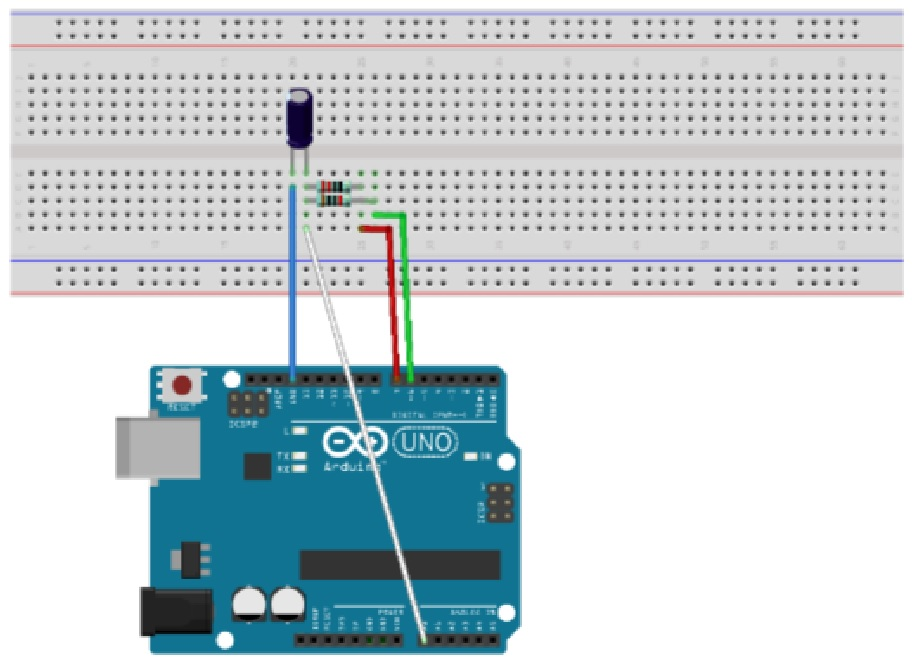
\includegraphics[scale = 0.35]{schemat.jpg}
		\caption{Układ RC wykorzystywany do przeprowadzenia pomiarów}
	\end{figure}
	Zostało wykonanych 12. pomiarów, cztery dla~każdego z~trzech kondensatorów o~wartościach $10\mu F, 100\mu F$ oraz $470\mu F$. Użyte zostały konretne wartości parametrów $\alpha$ i $\beta$ tak, by $\alpha+\beta=1$:
	\begin{table}[h] %nie wiem czy to dobrze wygląda, więc feel free to change
		\centering
		\begin{tabular}{cc}
			\hline
			$\alpha$ & $\beta$ \\ \hline
			0.1 & 0.9  \\ \hline
			0.125 & 0.875  \\ \hline
			0.25 & 0.75 \\ \hline
			0.45 & 0.55  \\ \hline
		\end{tabular}
	\end{table}
	\section{Wyniki}
	\subsection{470}
	\begin{figure}[H]
		\centering
		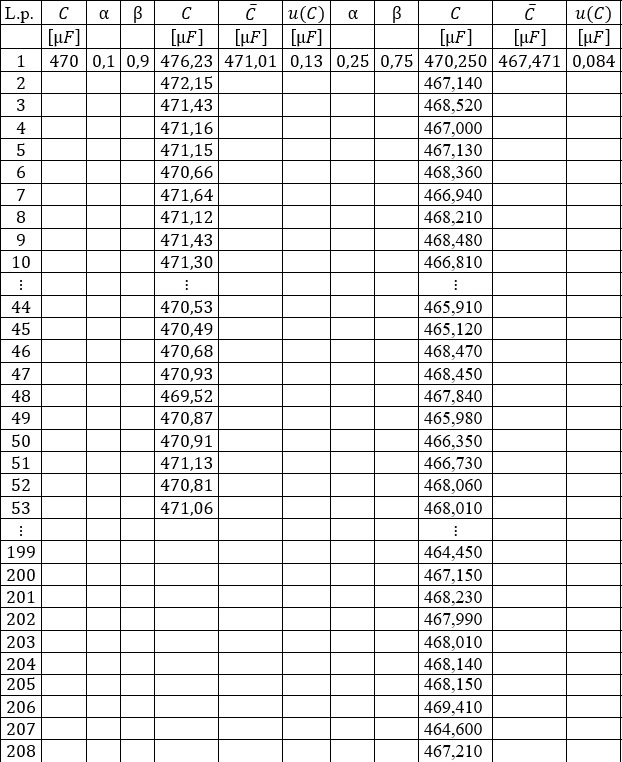
\includegraphics{470_tab_a.jpg}
	\end{figure}
	\begin{figure}[H]
		\centering
		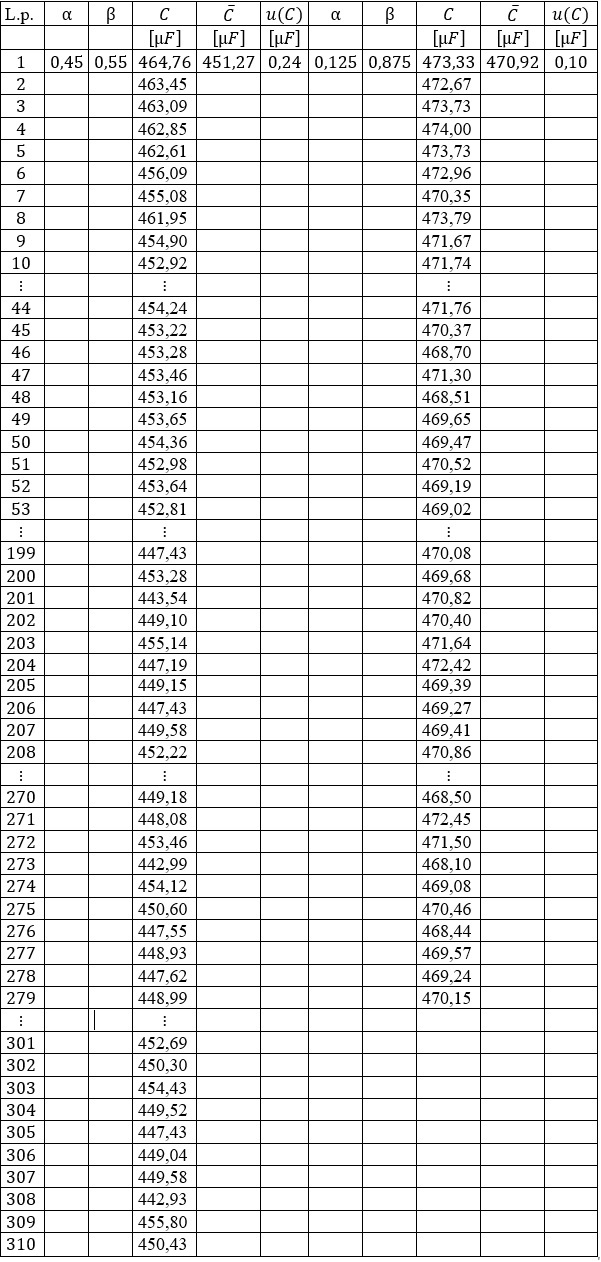
\includegraphics{470_tab_b.jpg}
	\end{figure}
	\subsection{100}
	\begin{figure}[H]
		\centering
		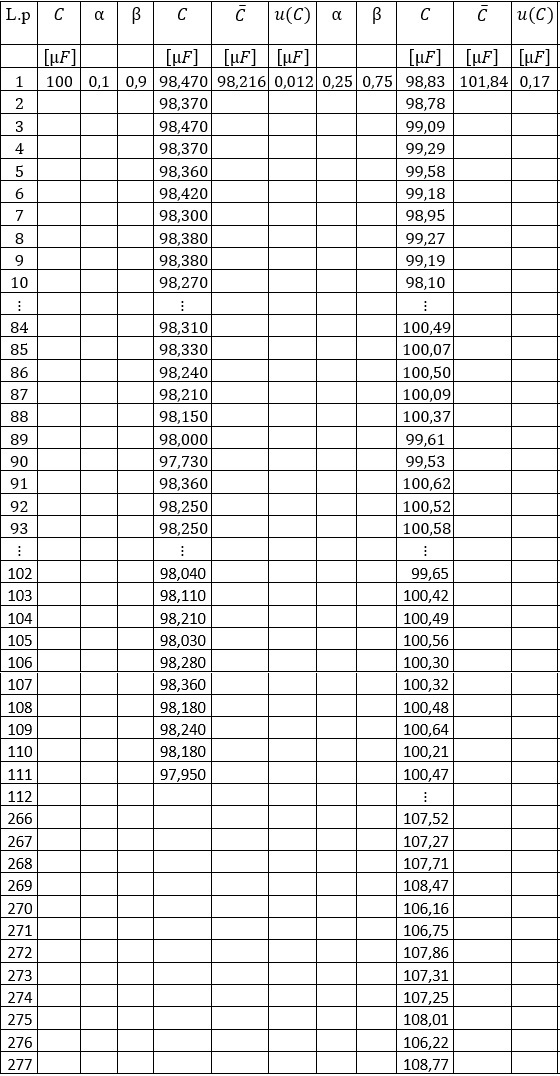
\includegraphics{100_tab_a.jpg}
	\end{figure}
	\begin{figure}[H]
		\centering
		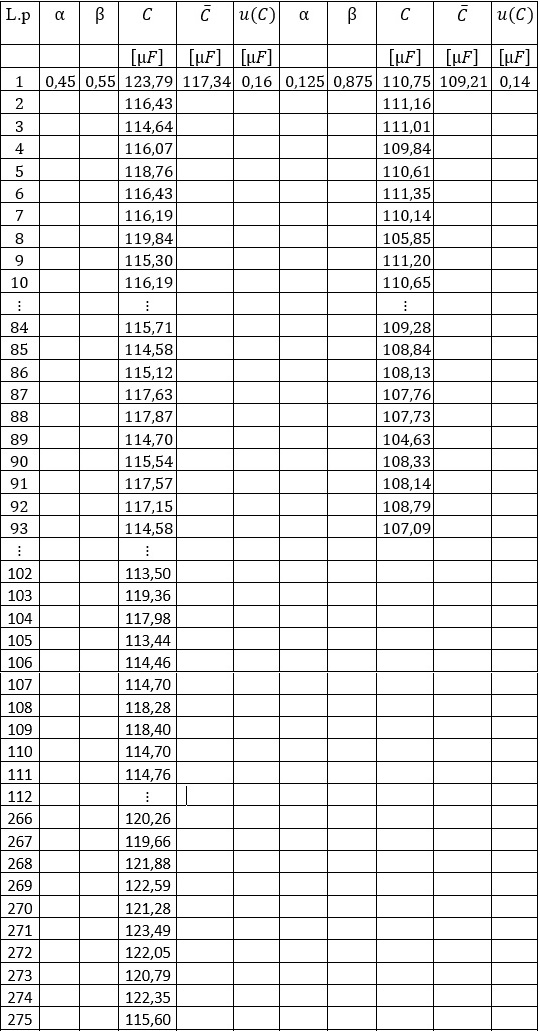
\includegraphics{100_tab_b.jpg}
	\end{figure}
	\subsection{10}
	\begin{figure}[H]
		\centering
		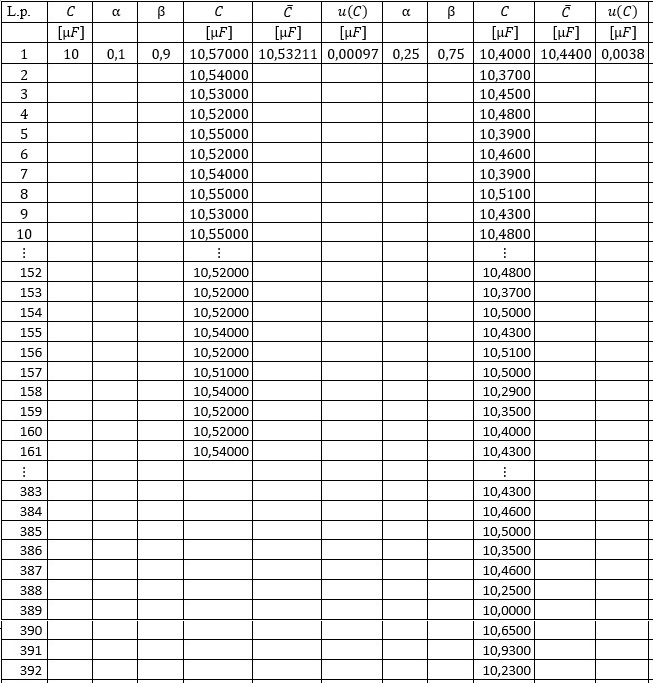
\includegraphics{10_tab_a.jpg}
	\end{figure}
	\begin{figure}[H]
		\centering
		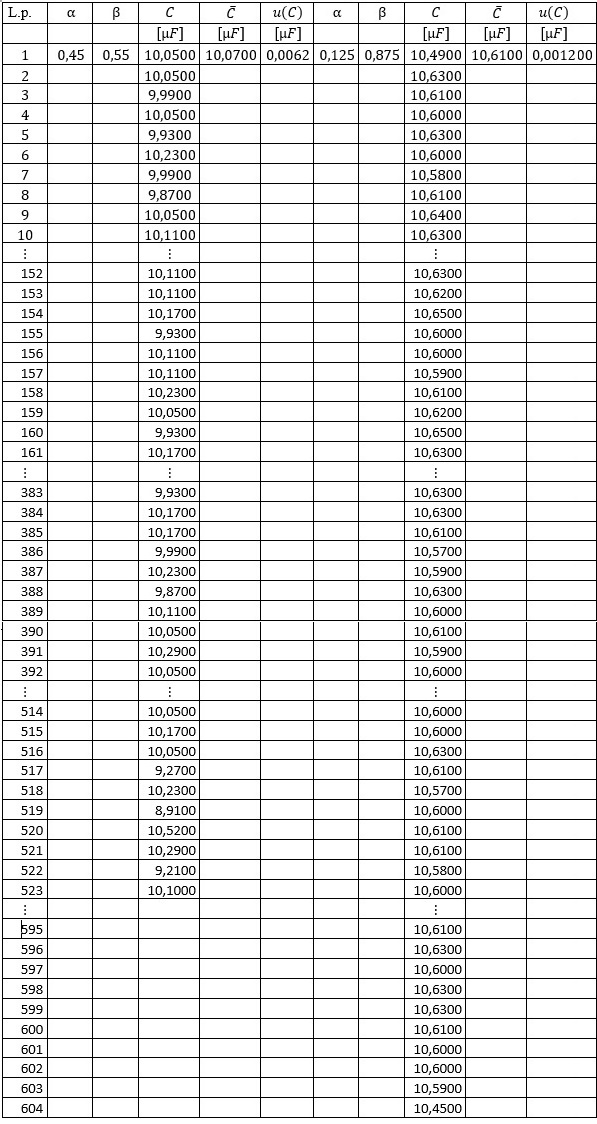
\includegraphics{10_tab_b.jpg}
	\end{figure}
	\section{Obliczenia}
	\subsection{Średnia}
	\subsubsection{Wzór}
	\begin{equation}
		\bar X = \frac{1}{n}\sum\limits_{i=1}^{n} X_{i},
	\end{equation}
	gdzie $i=1,2,3,\dots ,n, X_{i},$ to pojedyncza obserwacja, a $n$, to ilość/liczba obserwacji
	\subsubsection{Przykładowe obliczenia}
	dla $C=470\mu F, \alpha=0,1, \beta=0,9, n=53$
	\begin{equation}
		\bar C = \frac{1}{53}\sum\limits_{i=1}^{53} C_{i}=\frac{476,23\mu F+472,15\mu F+471,43\mu F+\dots +471,06\mu F}{53}\approx471,01\mu F
	\end{equation}
	\subsection{Niepewność typu A}
	\subsubsection{Wzór}
	\begin{equation}
		u_{A}\left(X\right)=\sqrt{\frac{\sum\limits_{i=1}^{n}{\left(X_{i}-\bar X\right)}^2}{n\left(n-1\right)}}
	\end{equation}
	\subsubsection{Przykładowe obliczenia}
	dla $C=470\mu F, \alpha=0,1, \beta=0,9, n=53, \bar C=471,01\mu F$
	\begin{multline}
		u_{A}\left(C\right)=\sqrt{\frac{\sum\limits_{i=1}^{53}{\left(C_{i}-\bar C\right)}^2}{53\left(53-1\right)}}=\\ \sqrt{\frac{{\left(476,23\mu F-471,01\mu F\right)}^2+{\left(472,15\mu F-471,01\mu F\right)}^2+\dots +{\left(476,23\mu F-471,06\mu F\right)}^2}{53\cdot 52}}\approx0,13\mu F
	\end{multline}
	\subsection{Porównanie empirycznych i teoretycznych pojemności kondensatora}:
	\begin{itemize}
		\item[$\bullet$] dla $\alpha=0,1$ i $\beta=0,9$:
		\begin{table}[h]
			\centering
			\begin{tabular}{cc}
				\hline
				$C$ teoretyczne & $C$ empiryczne \\ \hline
				$\mu F$ & $\mu F$ \\ \hline
				$10$ & $10,53211\pm0,00097$  \\ \hline
				$100$ & $98,216\pm0,012$  \\ \hline
				$470$ & $471,01\pm0,13$  \\ \hline
			\end{tabular}
		\end{table}
		\item[$\bullet$] dla $\alpha=0,125$ i $\beta=0,875$:
		\begin{table}[h]
			\centering
			\begin{tabular}{cc}
				\hline
				$C$ teoretyczne & $C$ empiryczne \\ \hline
				$\mu F$ & $\mu F$ \\ \hline
				$10$ & $10,6100\pm0,0012$  \\ \hline
				$100$ & $109,21\pm0,14$  \\ \hline
				$470$ & $470,92\pm0,10$  \\ \hline
			\end{tabular}
		\end{table}
		\item[$\bullet$] dla $\alpha=0,25$ i $\beta=0,75$:
		\begin{table}[H]
			\centering
			\begin{tabular}{cc}
				\hline
				$C$ teoretyczne & $C$ empiryczne \\ \hline
				$\mu F$ & $\mu F$ \\ \hline
				$10$ & $10,4400\pm0,0038$  \\ \hline
				$100$ & $101,84\pm0,55$  \\ \hline
				$470$ & $467,471\pm0,084$  \\ \hline
			\end{tabular}
		\end{table}
		\item[$\bullet$] dla $\alpha=0,45$ i $\beta=0,55$:
		\begin{table}[h]
			\centering
			\begin{tabular}{cc}
				\hline
				$C$ teoretyczne & $C$ empiryczne \\ \hline
				$\mu F$ & $\mu F$ \\ \hline
				$10$ & $10,0700\pm0,0062$  \\ \hline
				$100$ & $117,34\pm0,16$  \\ \hline
				$470$ & $451,27\pm0,24$  \\ \hline
			\end{tabular}
		\end{table}
	\end{itemize}
	\section{Wykresy}
	\subsection{Naładowanie i rozładowanie kondensatora}:
	
	\subsection{Pojemność kondensatora: $10 \mu F$}
	\begin{figure}[H]
		\centering
		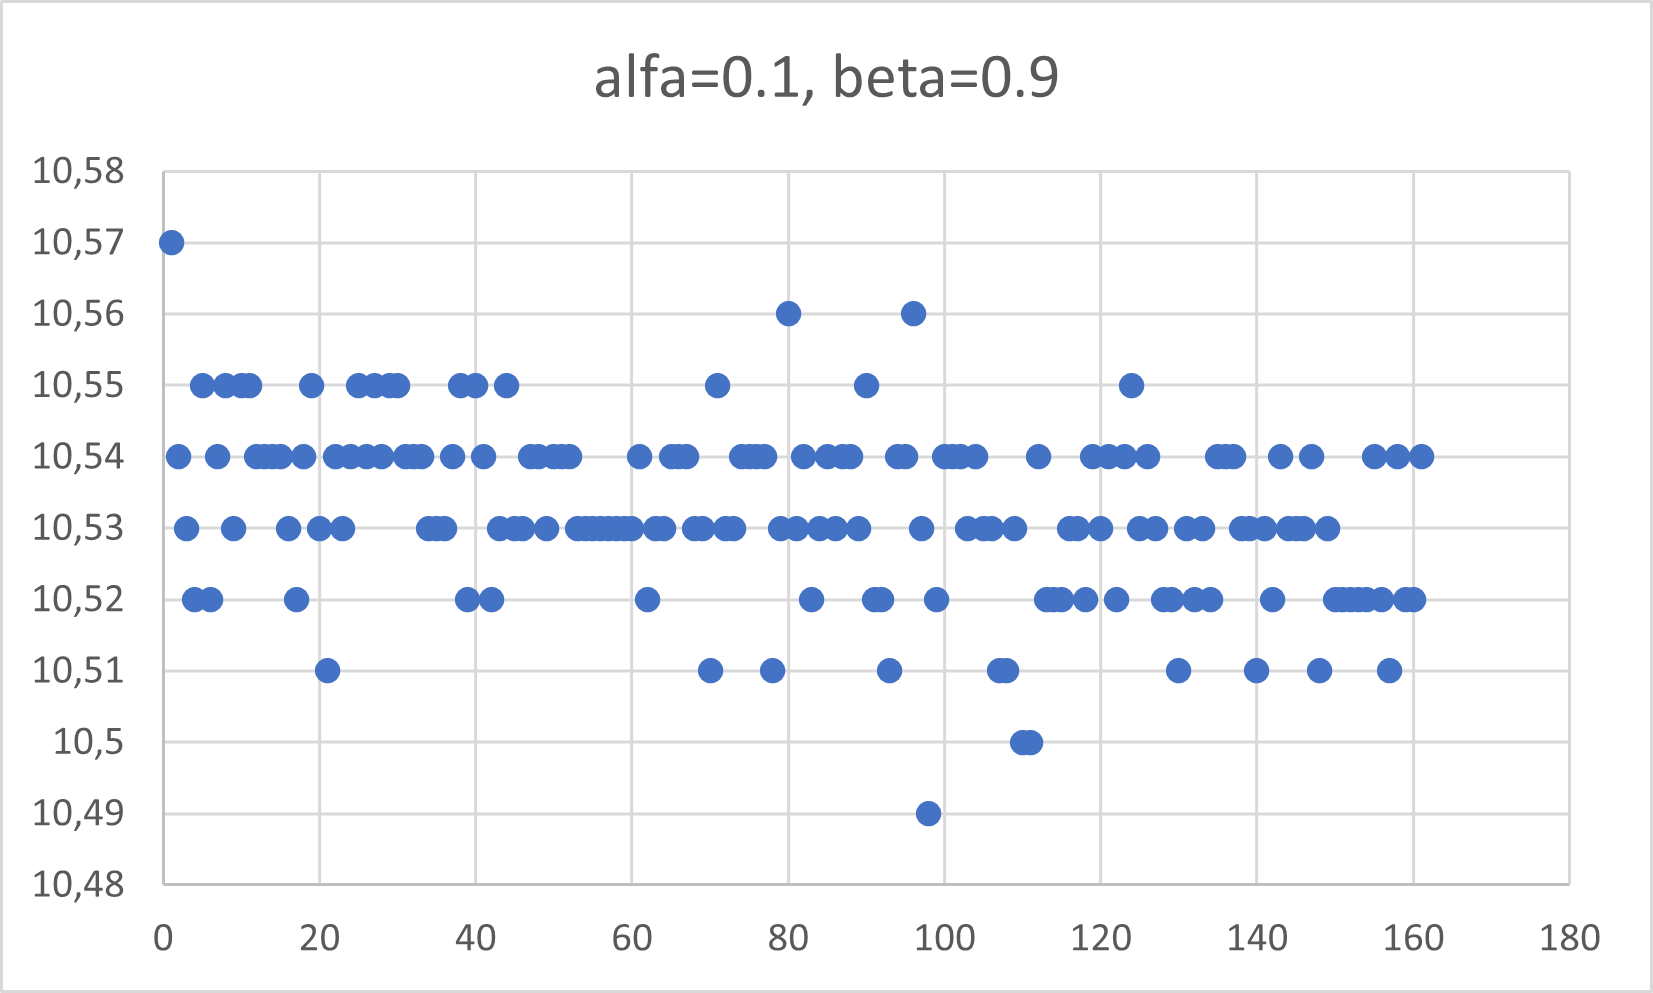
\includegraphics{10_a0.1.png}
	\end{figure}
	\begin{figure}[H]
		\centering
		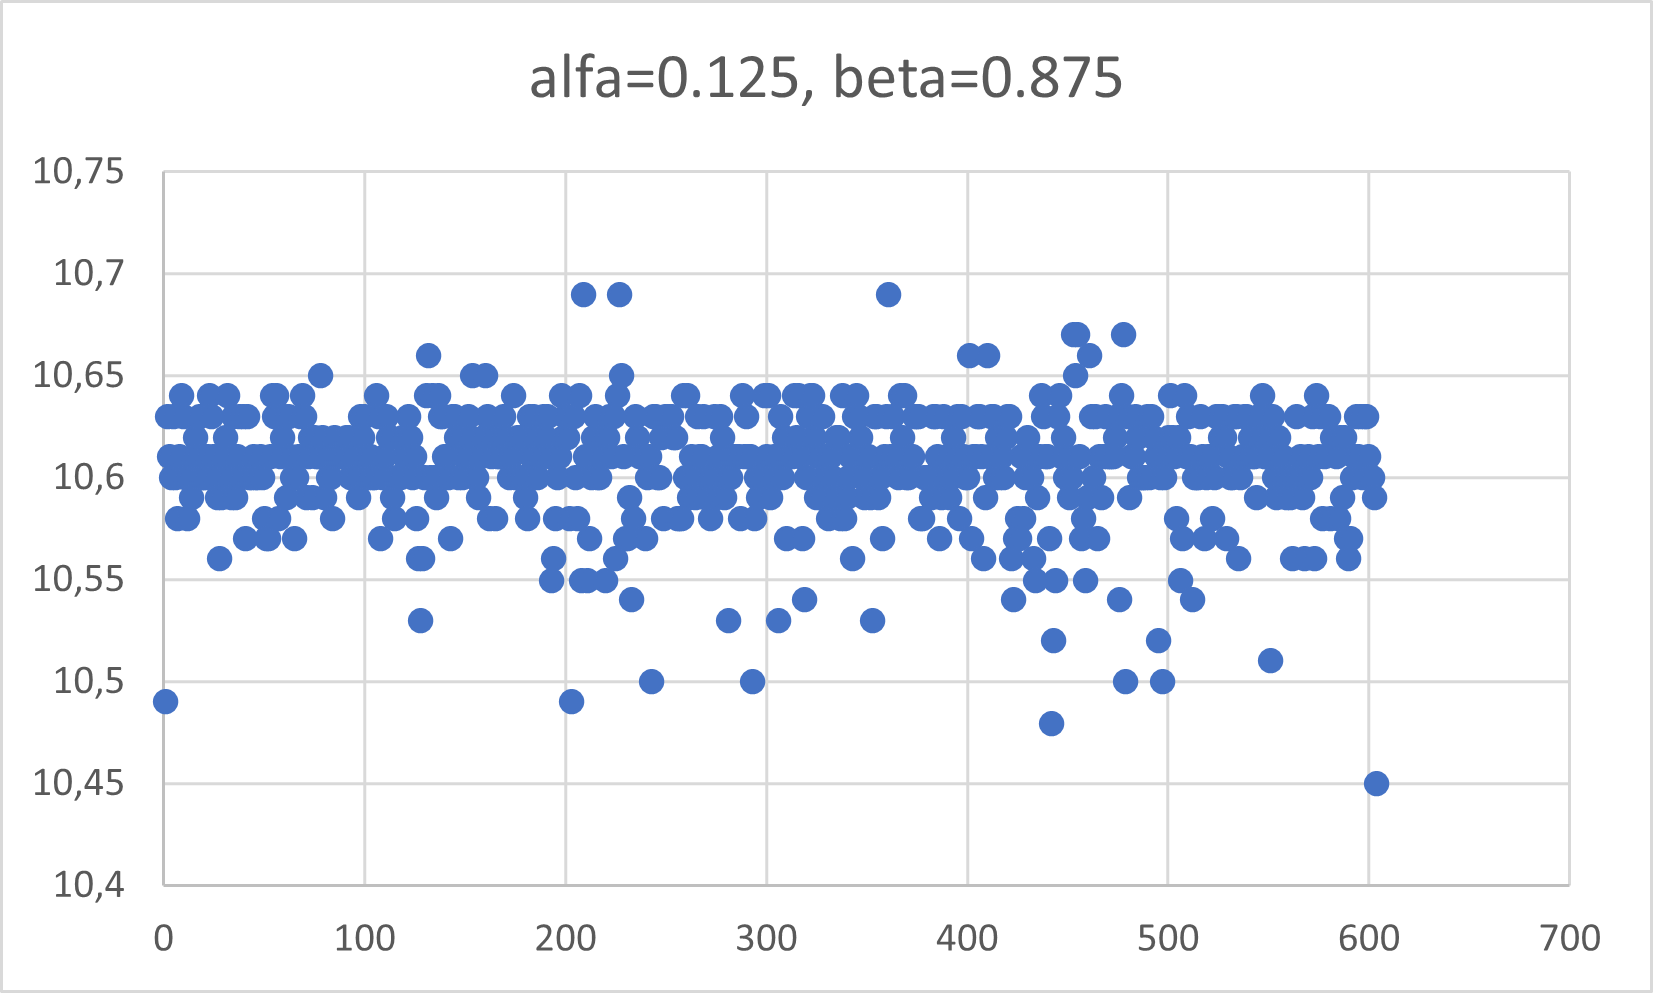
\includegraphics{10_a0.125.png}
	\end{figure}
	\begin{figure}[H]
		\centering
		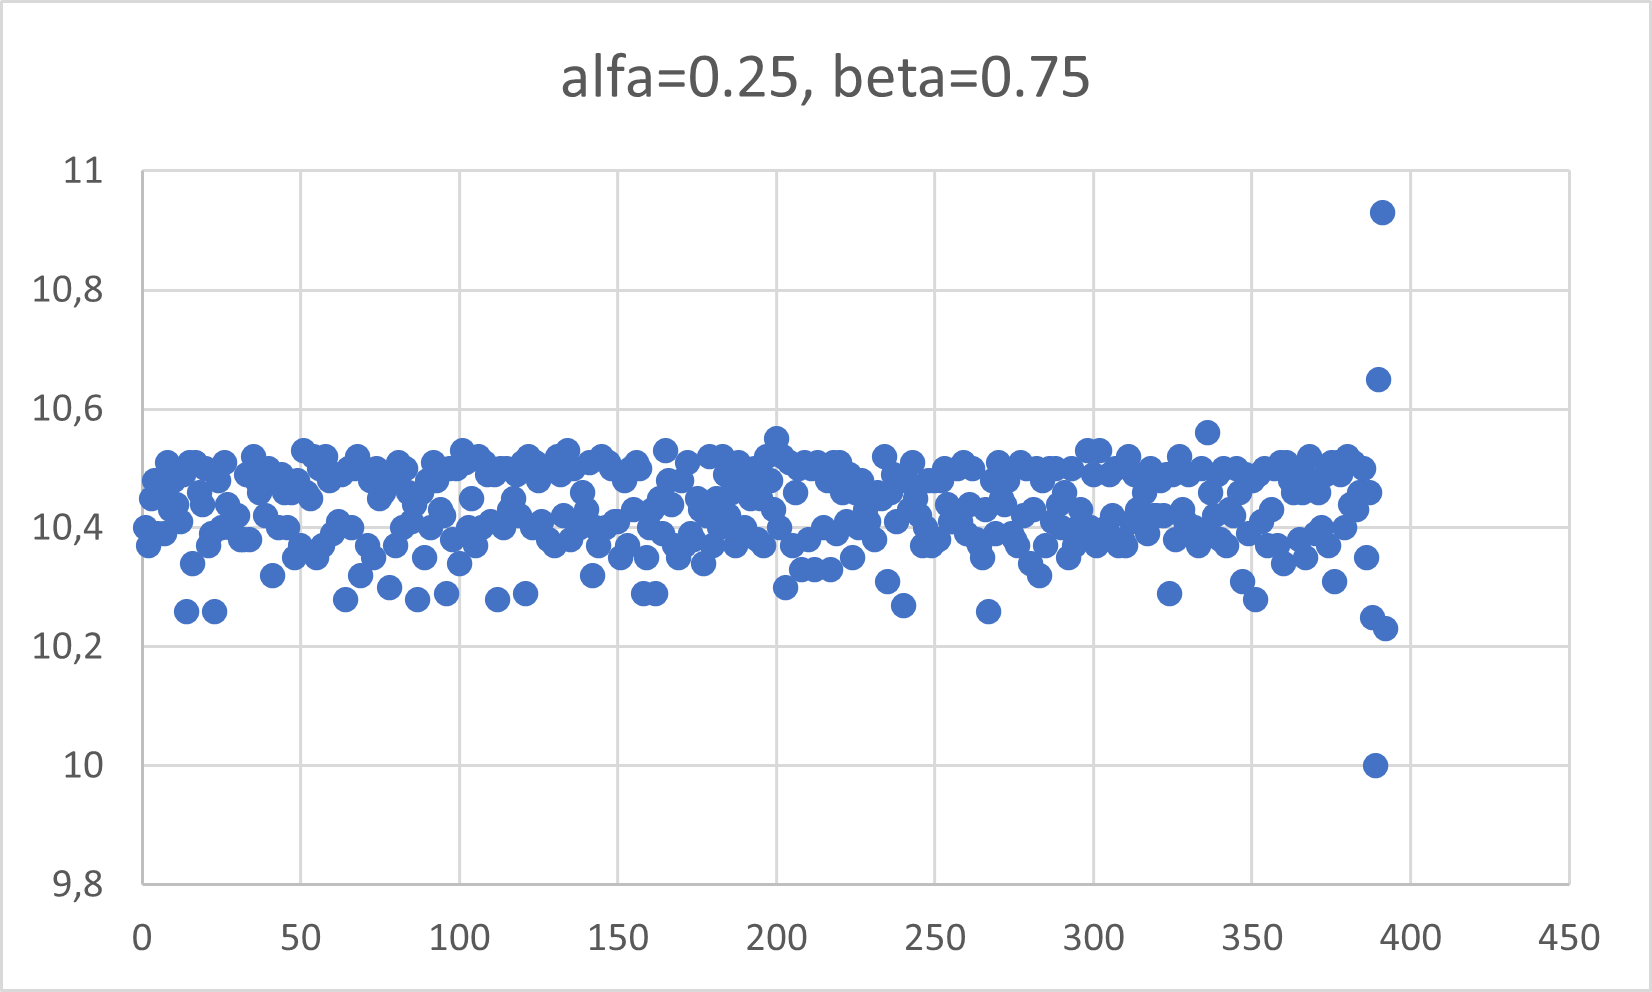
\includegraphics{10_a0.25.png}
	\end{figure}
	\begin{figure}[H]
		\centering
		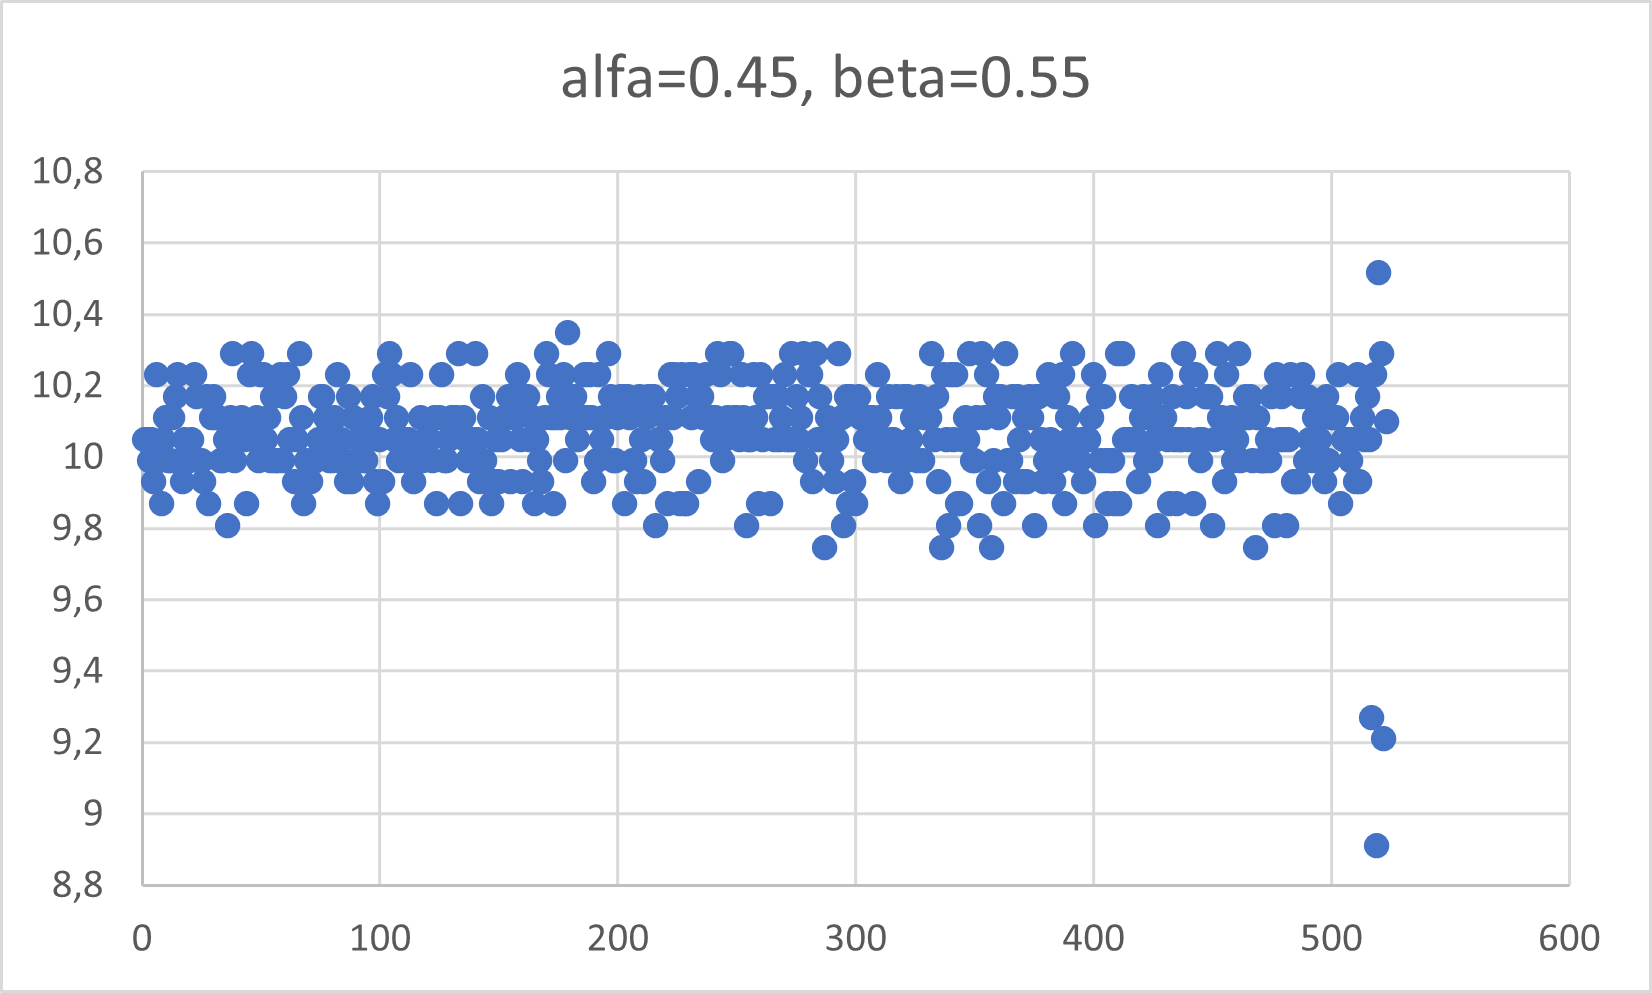
\includegraphics{10_a0.45.png}
	\end{figure}
	\subsection{Pojemność kondensatora: $100 \mu F$}
	\begin{figure}[H]
		\centering
		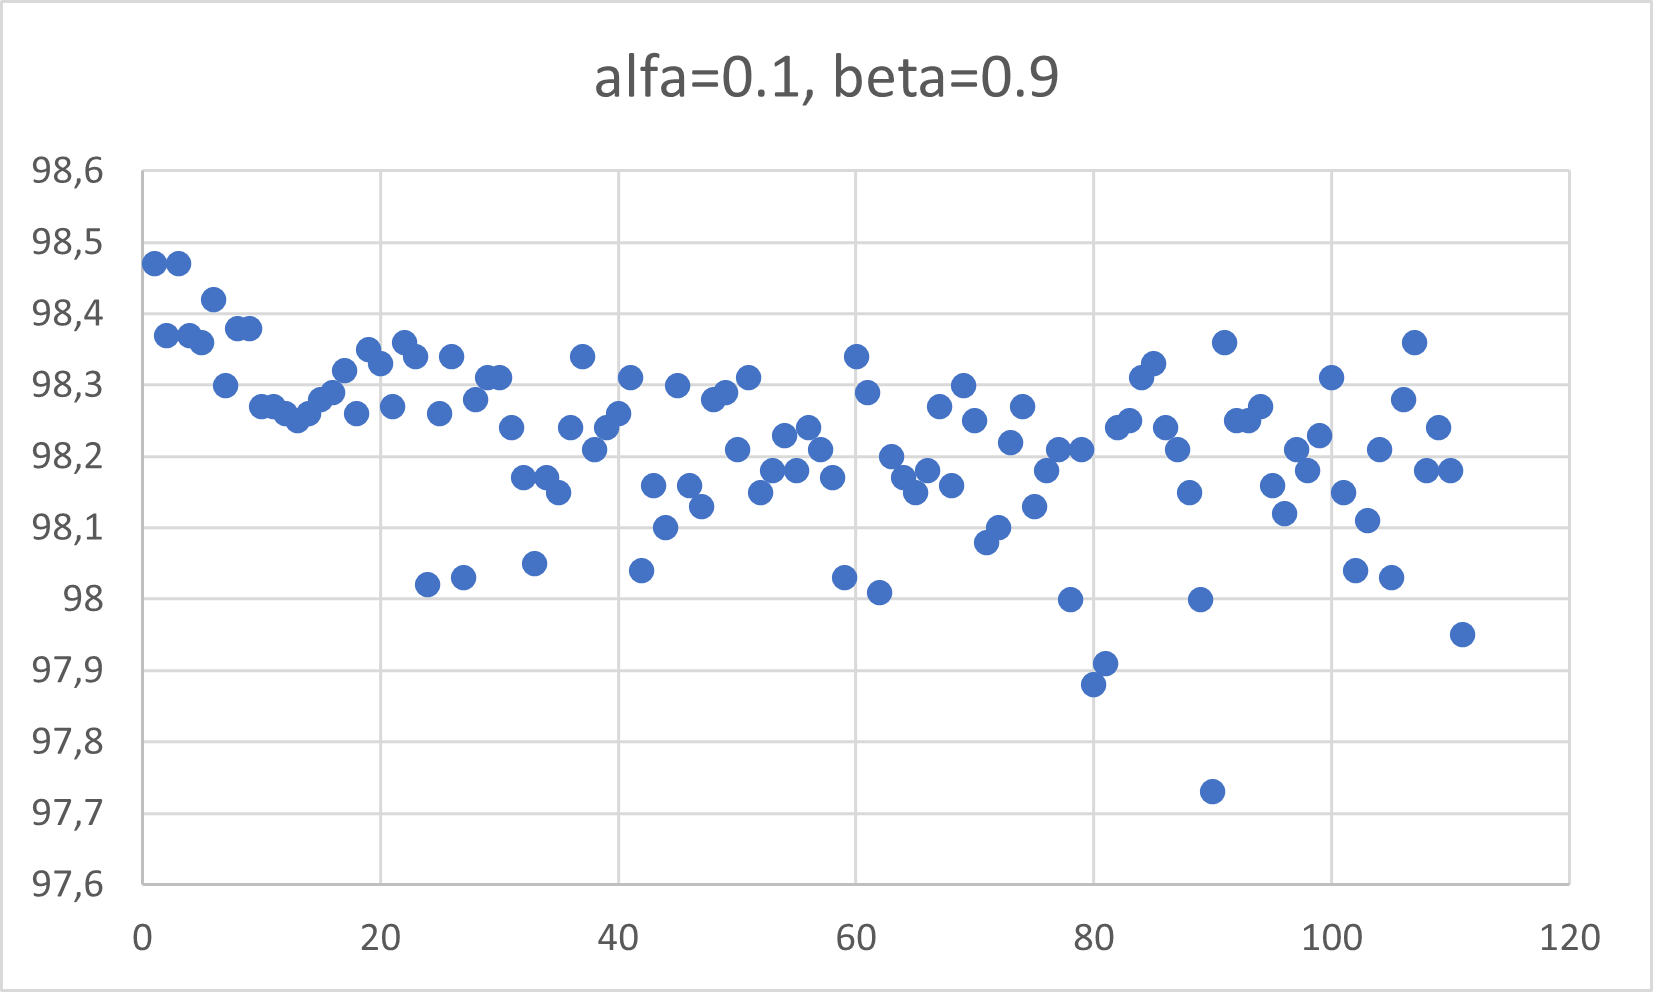
\includegraphics{100_a0.1.png}
	\end{figure}
	\begin{figure}[H]
		\centering
		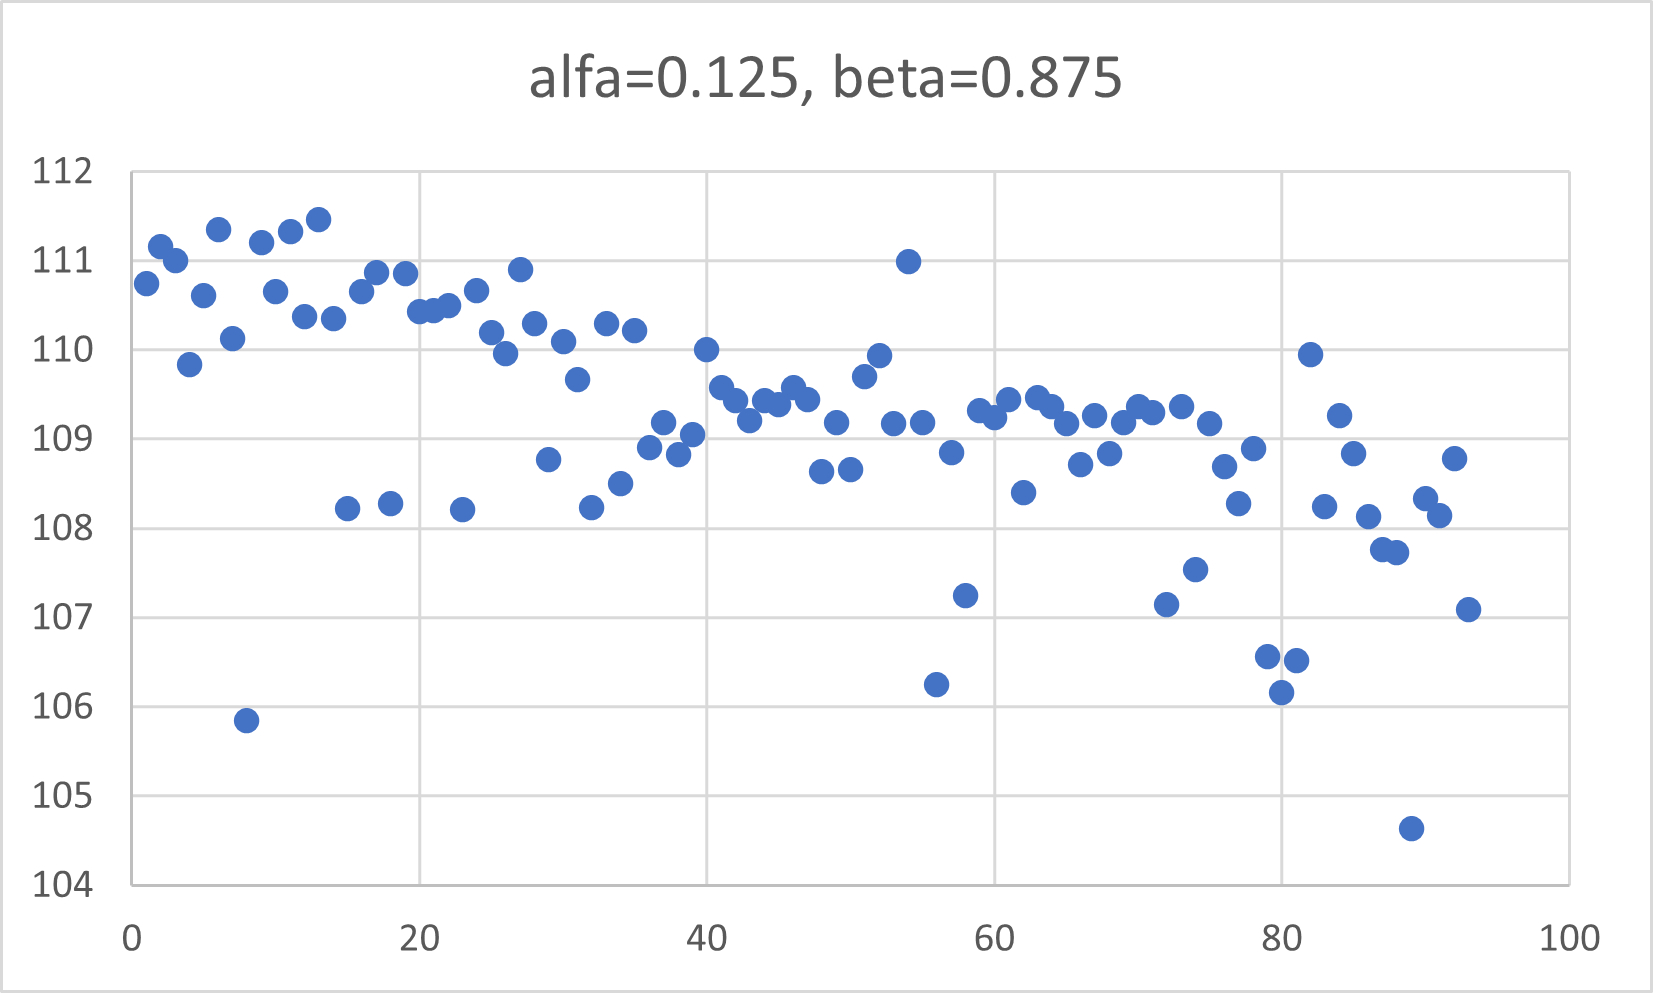
\includegraphics{100_a0.125.png}
	\end{figure}
	\begin{figure}[H]
		\centering
		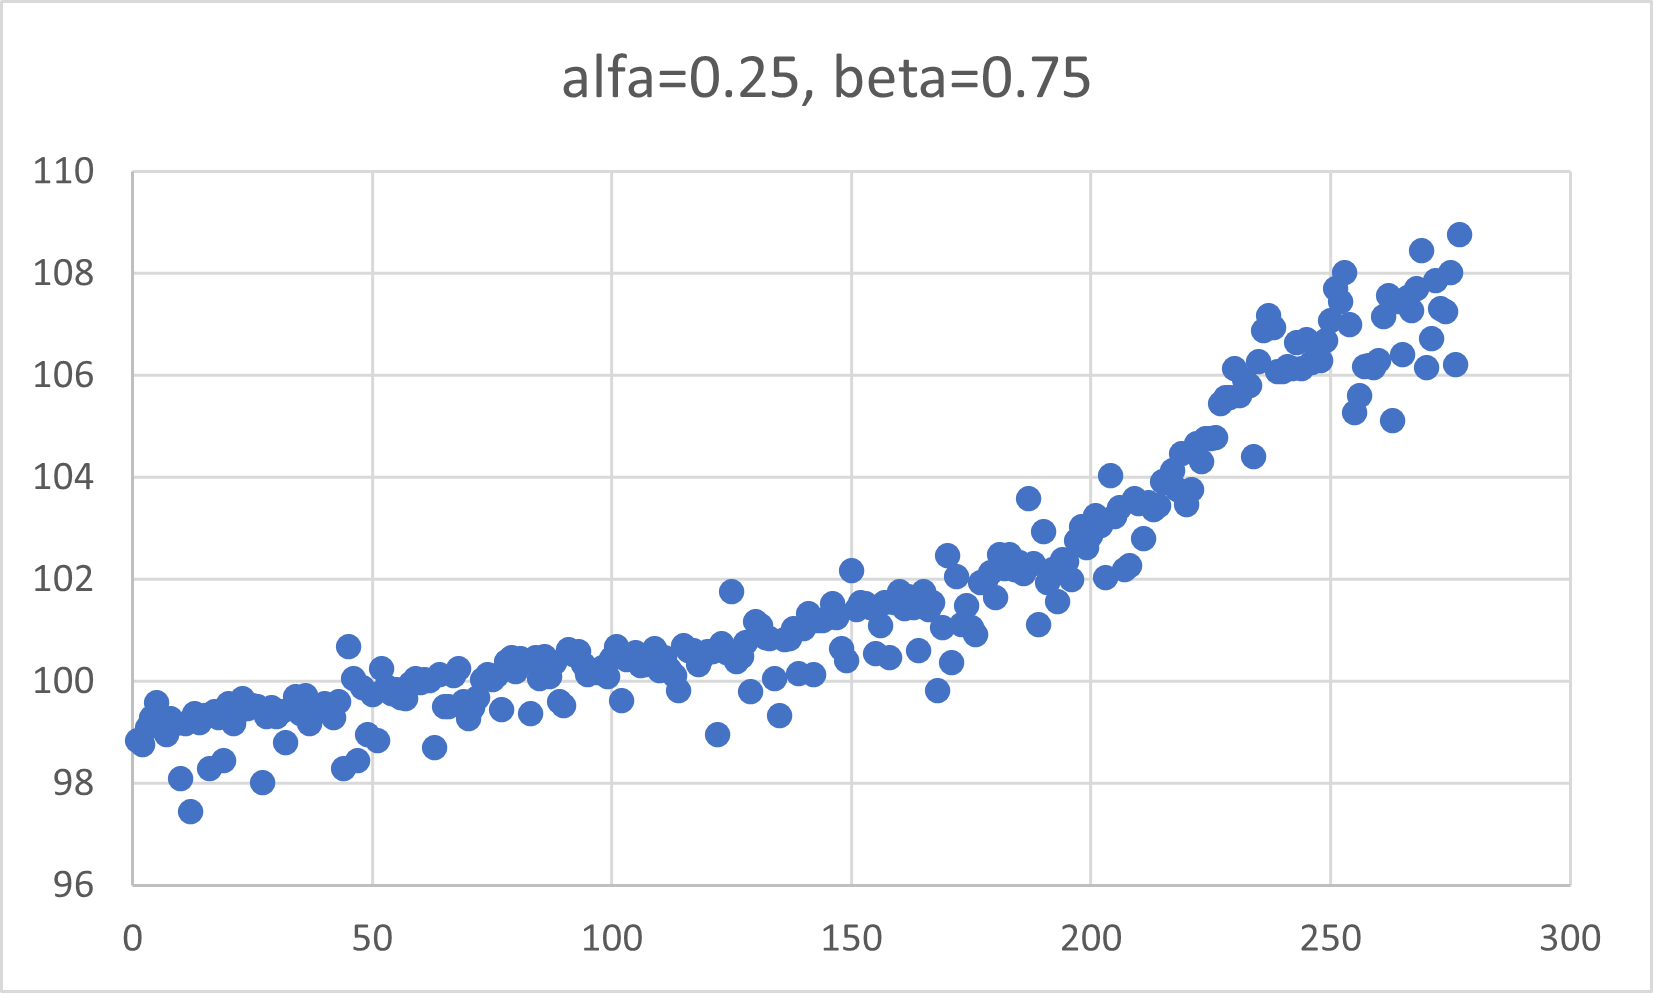
\includegraphics{100_a0.25.png}
	\end{figure}
	\begin{figure}[H]
		\centering
		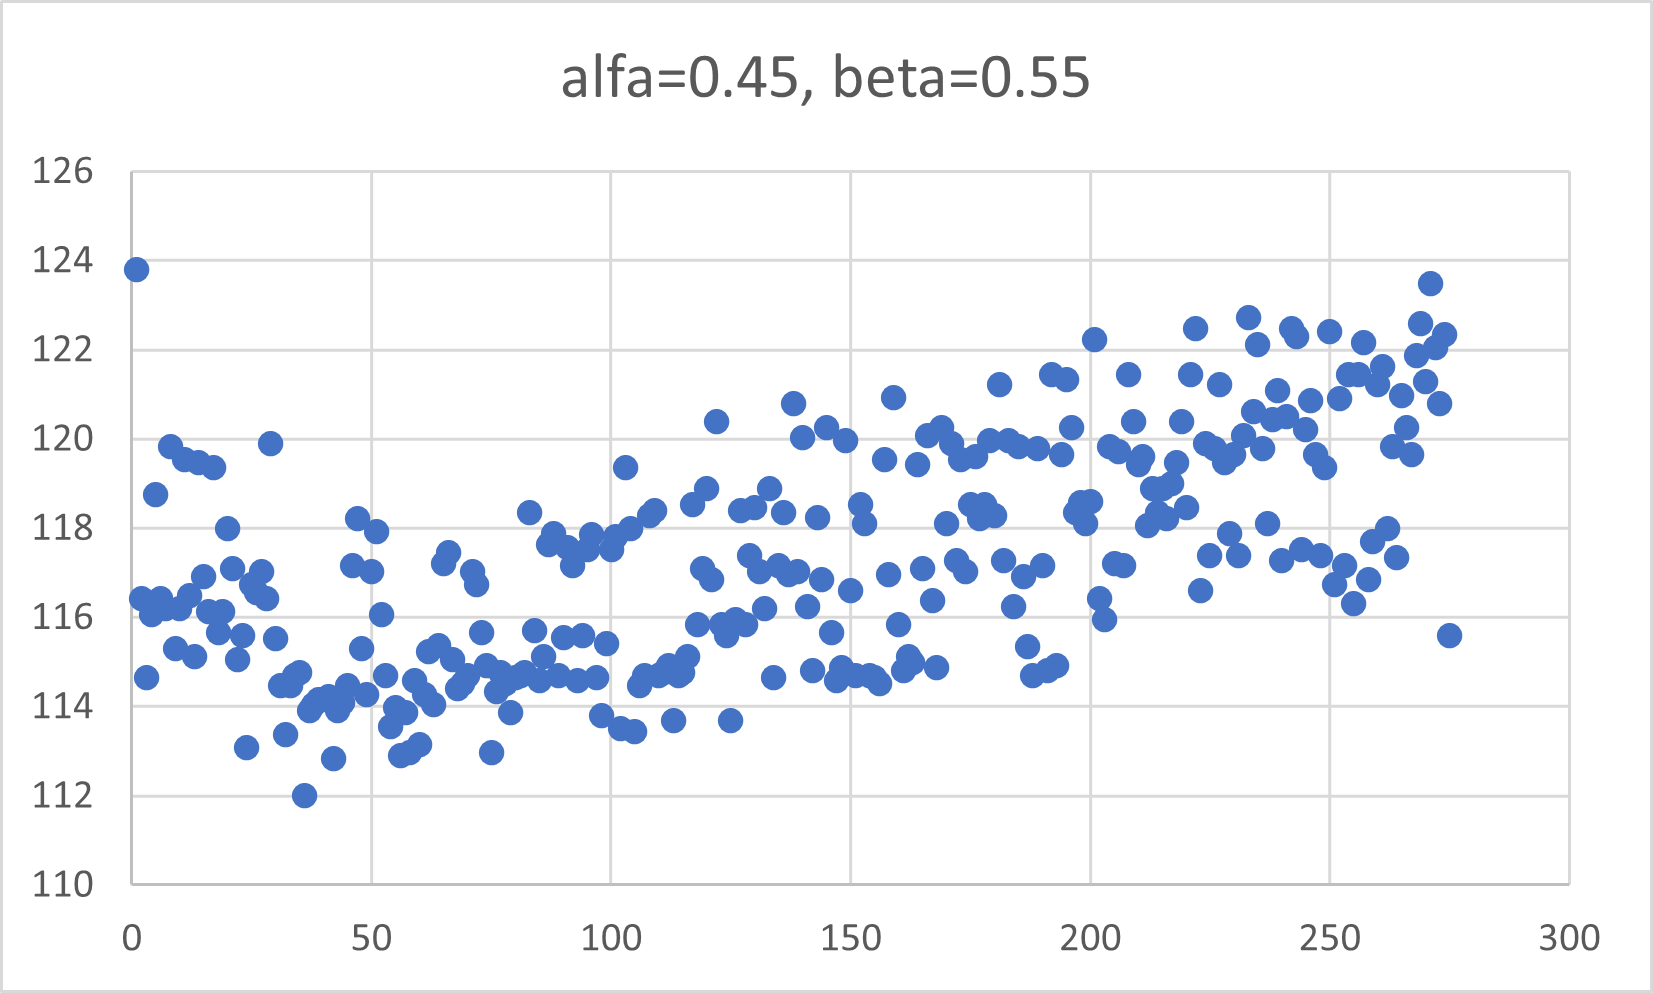
\includegraphics{100_a0.45.png}
	\end{figure}
	\subsection{Pojemność kondensatora: $470 \mu F$}
	\begin{figure}[H]
		\centering
		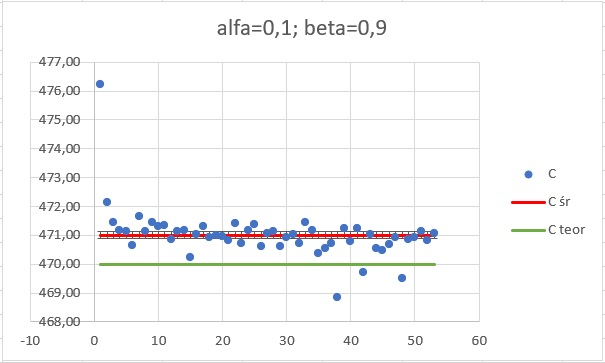
\includegraphics{470_a01.jpg}
	\end{figure}
	\begin{figure}[H]
		\centering
		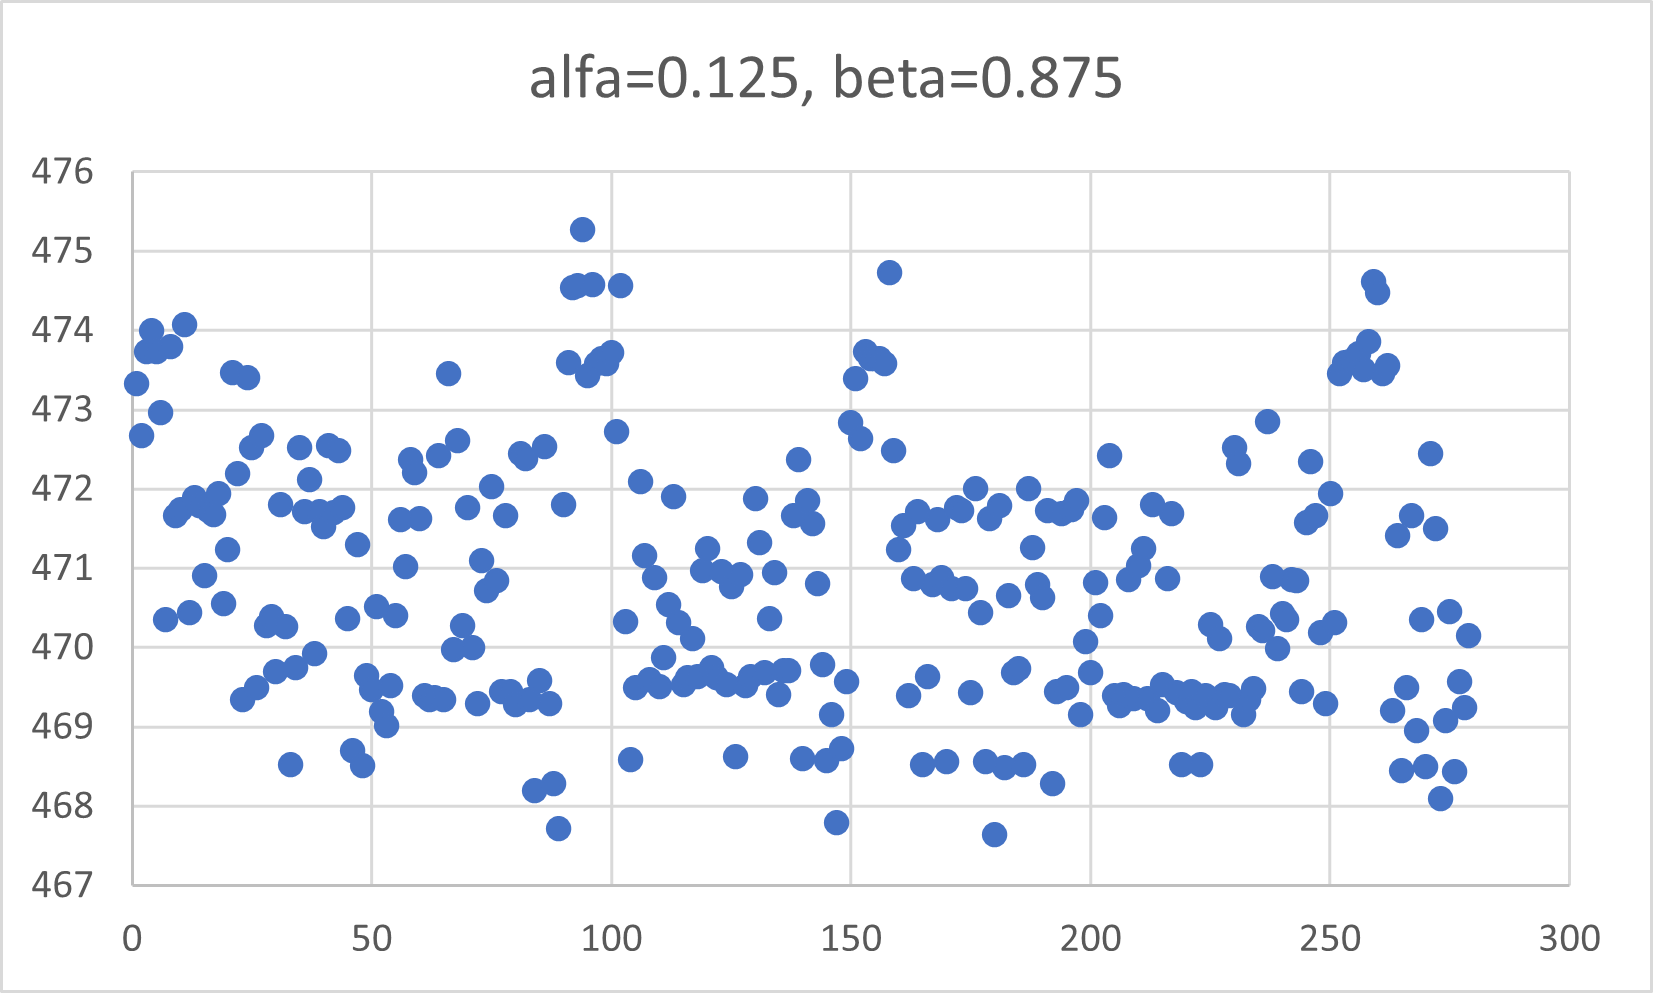
\includegraphics{470_a0.125.png}
	\end{figure}
	\begin{figure}[H]
		\centering
		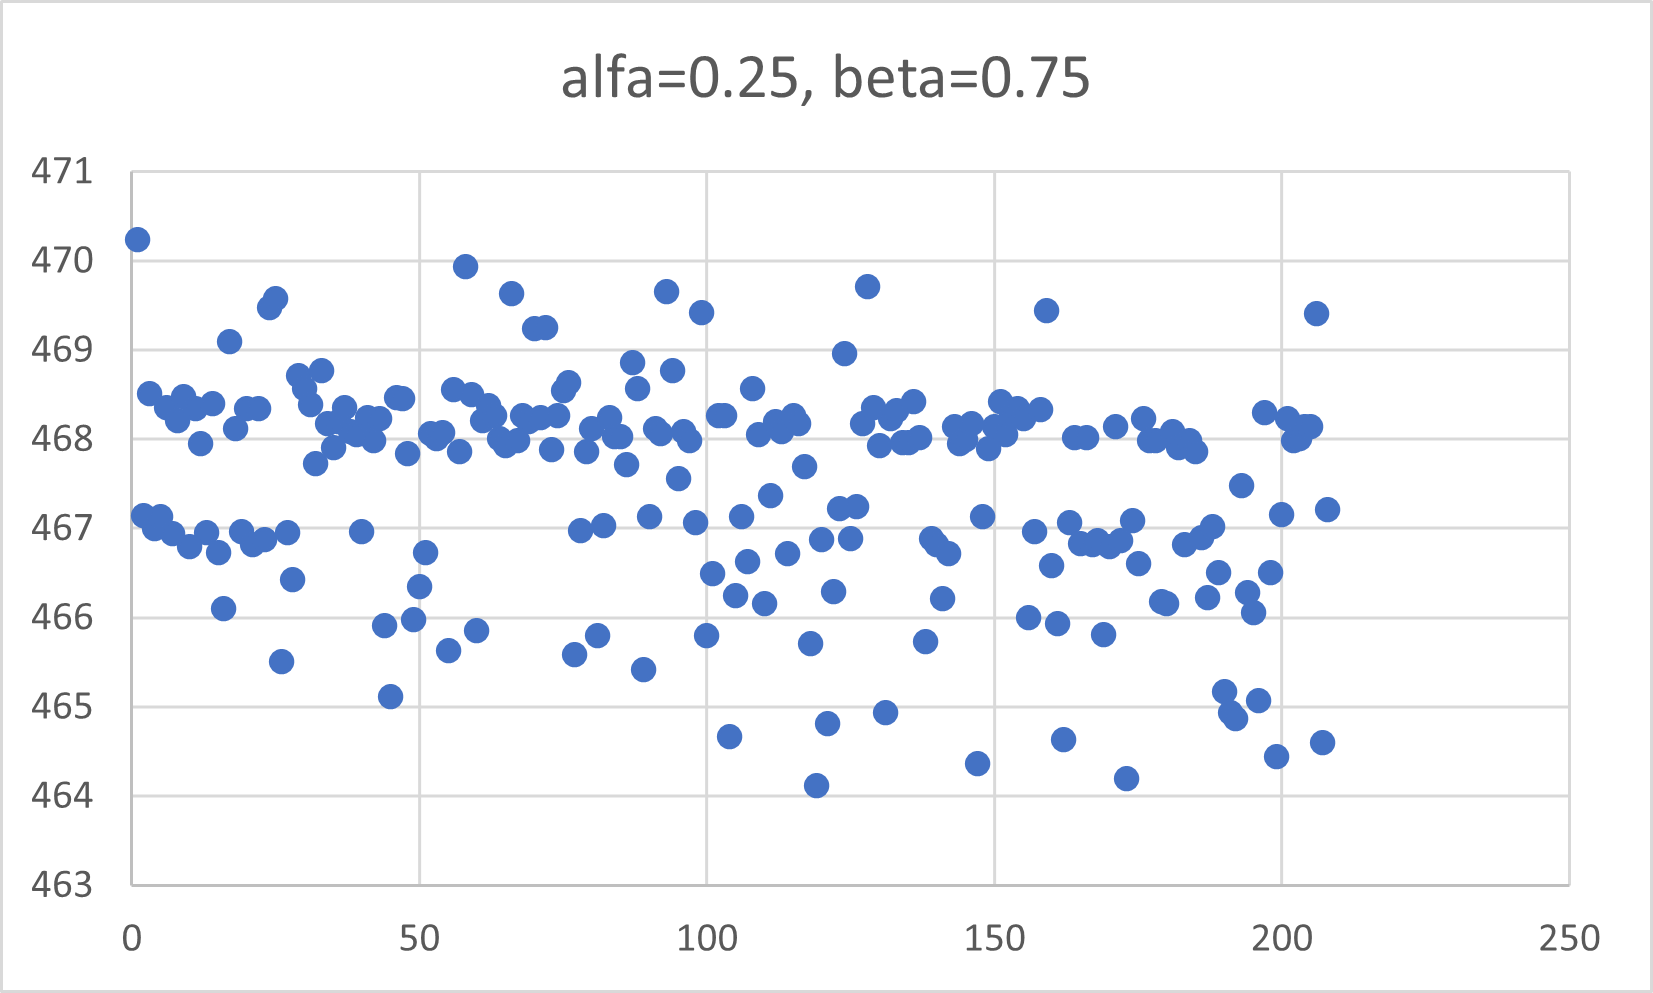
\includegraphics{470_a0.25.png}
	\end{figure}
	\begin{figure}[H]
		\centering
		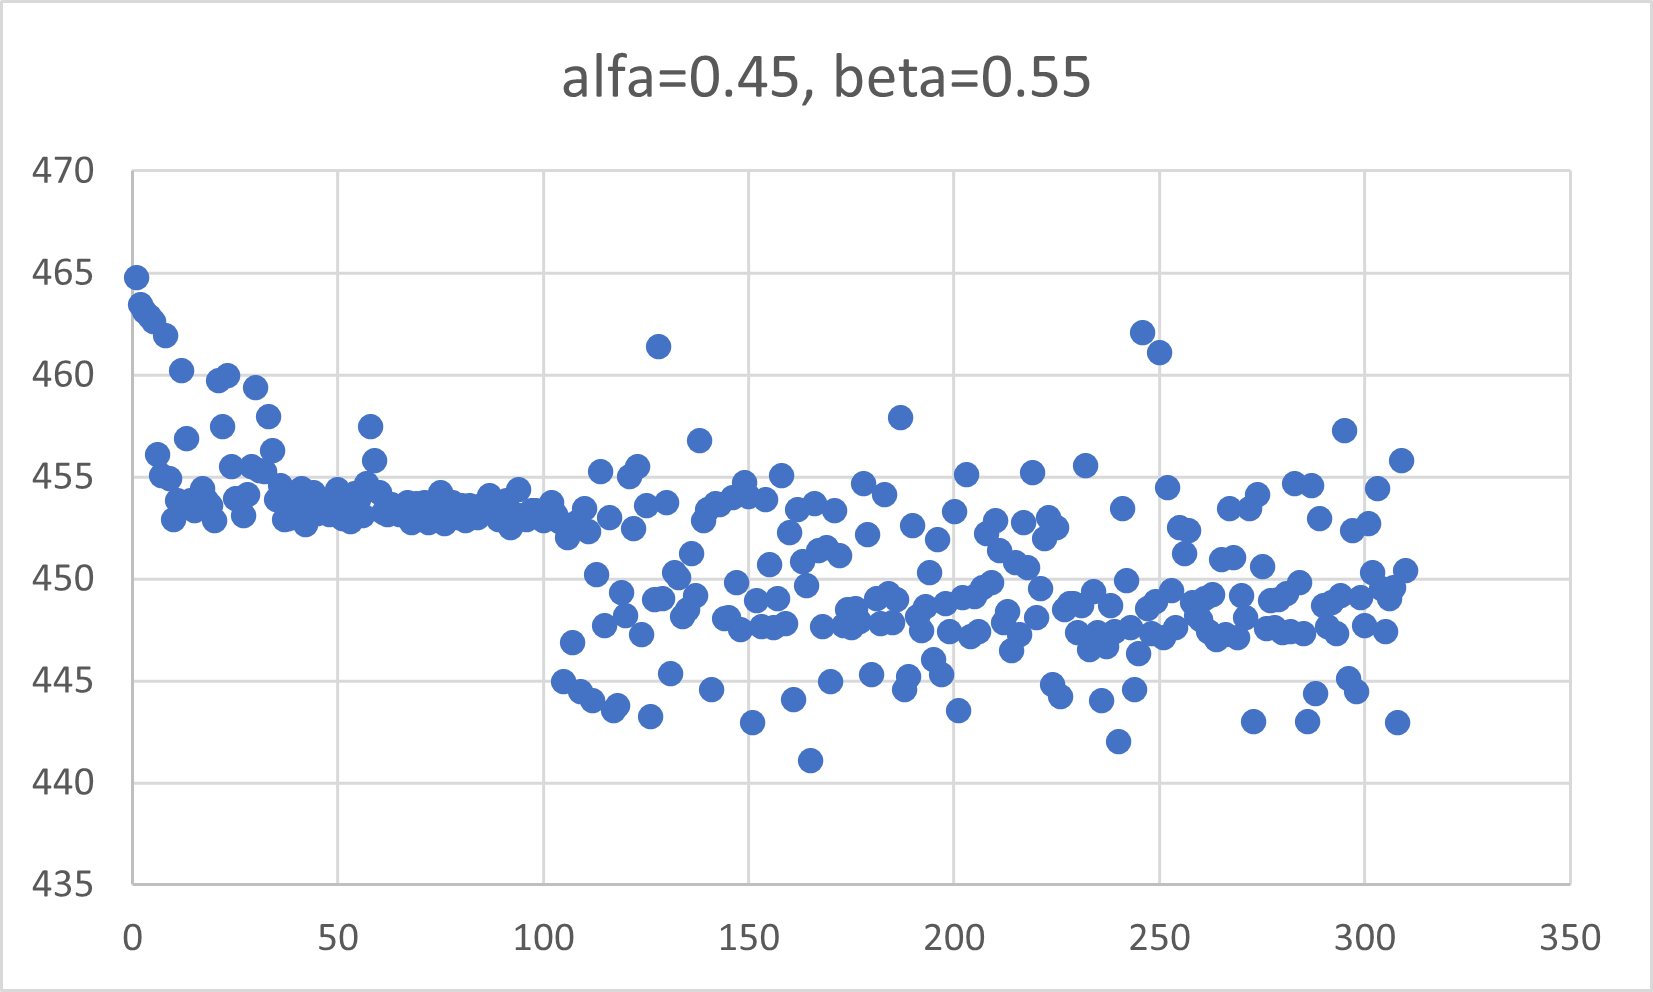
\includegraphics{470_a0.45.png}
	\end{figure}
	\section{Wnioski}
	\begin{itemize}
		\item[$\bullet$] Możemy zauważyć, że pojemność empiryczna kondensatorów zwiększa się wraz ze wzrostem odległości między $\alpha$ i $\beta$
		\item %coś że w 10 alfa=0.1 mało pomiarów to niedokładne przybliżenie
	\end{itemize}
\end{document}